\section{Problem 1}

\subsection{Instruction}

Write a function in Matlab that simulates the train-horn-Doppler scenario
discussed in lecture. Assume that the train tracks are rectilinear.

Be sure to account for the nonzero time of flight $\delta t_{TOF}$ as discussed
in lecture. The effect of $\delta t_{TOF} > 0$ is that the stationary observer
will discern an $f_D$ at time $t_k$ that relates to the train’s line-of-sight
velocity at time $t_k − \delta t_{TOF}$. More precisely, the apparent frequency
of the train horn at the location of the observer at time $t_k$ is given by

\begin{equation}
	f_r(t_k) = \frac{f_c}{1 + \frac{v_{los}(t_k)}{v_s}}
\end{equation}

where $f_c$ is the nominal horn frequency, $v_{los}(t_k)$ is the line-of-sight
velocity at $t_k$, and $v_s$ is the speed of the signal in the medium. Note that
the line-of-sight geometry used to calculate $v_{los}(t_k)$  is between the
observer at time $t_k$ and the horn at time $t_k − \delta t_{TOF}$.

Download the audio file trainout.wav from Canvas. This file was created with the
following input argument values:

\begin{lstlisting}
  fh = 440;
  vTrain = 20;
  t0 = 0;
  x0 = 0;
  delt = 0.01;
  N = 1000;
  vs = 343;
\end{lstlisting}

Set up your simulator with these same values. Estimate the values of xObs and
dObs by adjusting them in your simulation until you get an apparent received
frequency profile that matches the one in the audio file.

\subsection{MATLAB code}

\lstinputlisting{simulateTrainDoppler.m}
\lstinputlisting{topSimulateTrainDoppler_temp.m}

\subsection{Result}

Analizing the given signal it's possible to manually tag the moment in which the
train passed in front of the receiver. Figure~\ref{fig:spectrogram_original}
shows how the power density is concentrated at higher frequency before 3.069 sec
and drops rapidly after that. This indicates the exact moment at which the train
passed infront of the receiver.

\begin{figure}[H]
	\centering
	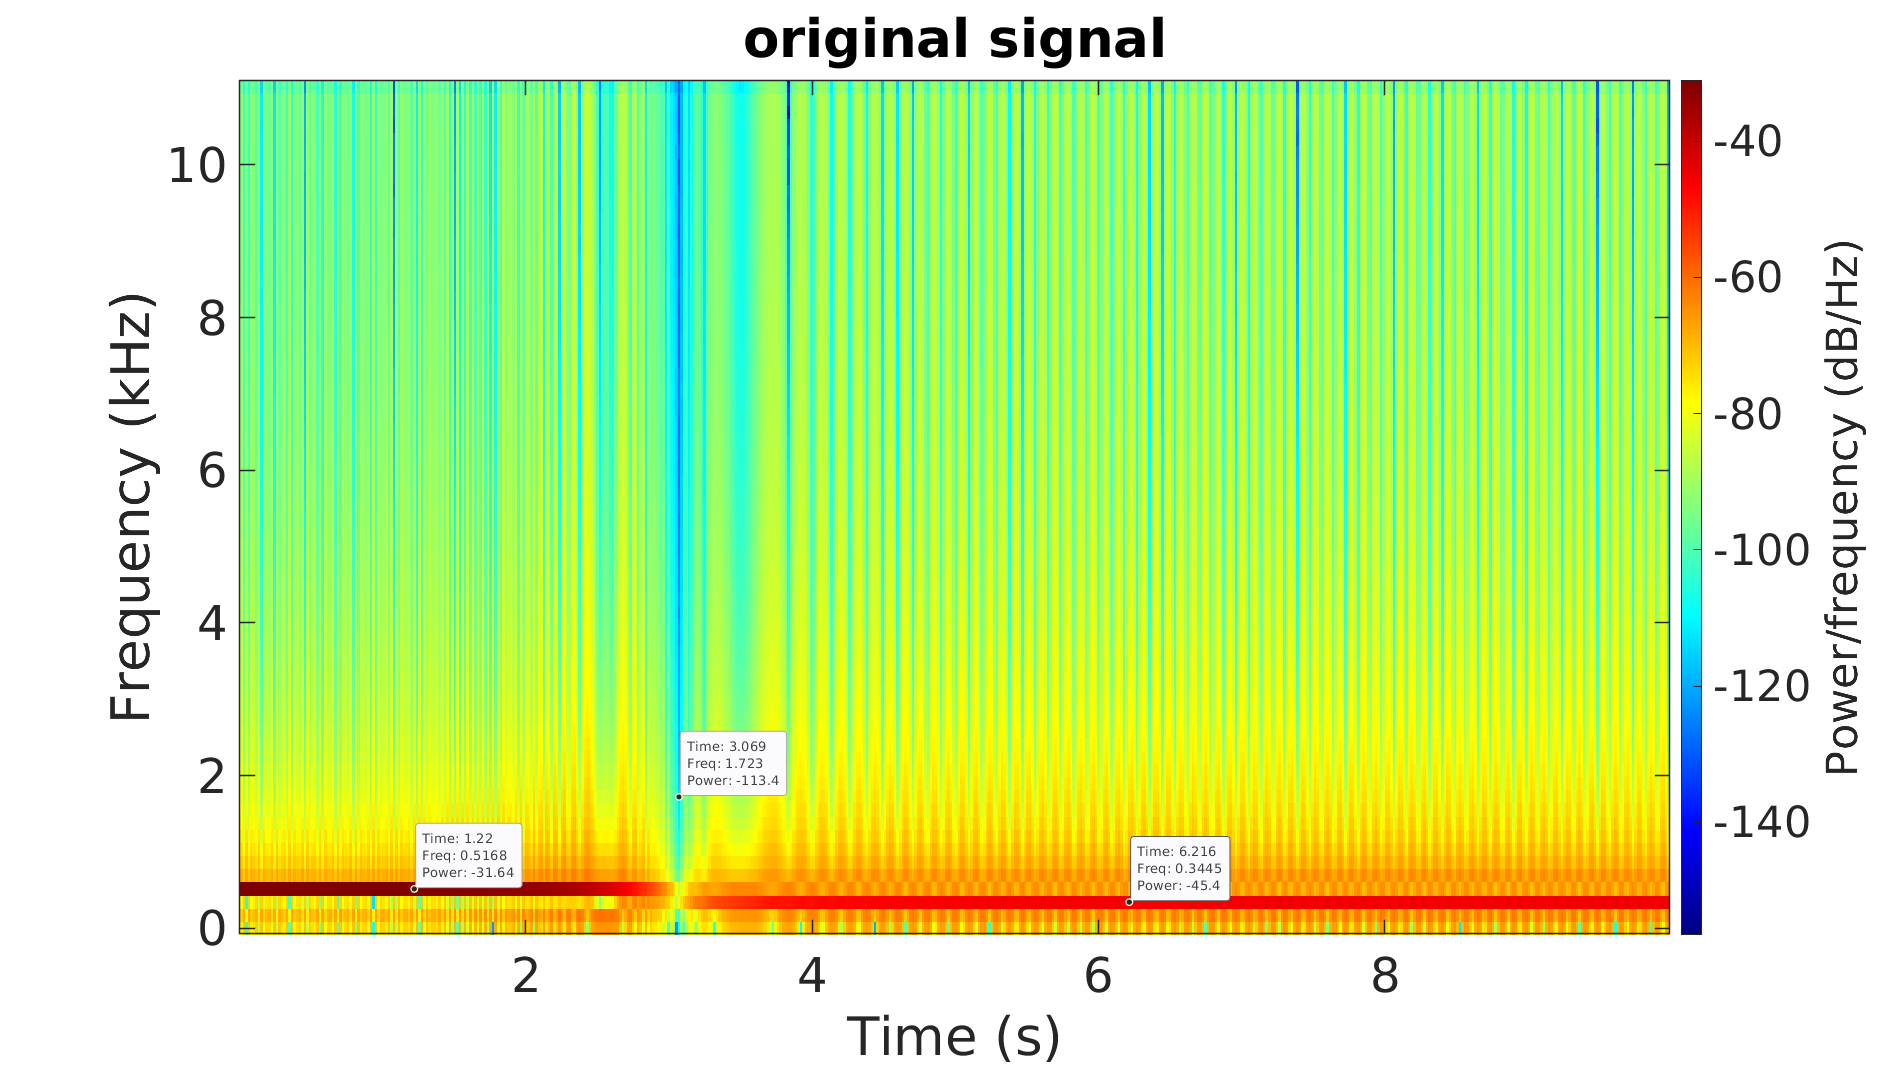
\includegraphics[width=0.9\textwidth]{figs/ex1_spectrogram_orig.png}
	\caption{Spectrogram of the given signal.}
	\label{fig:spectrogram_original}
\end{figure}

This, approach lead to $xObs = 56.8$ and $dObs = 10$.



